\selectlanguage{english}
\appendice{Probabilités de transition entre réseaux trophiques}
\label{annIII}
\addtocounter{chapter}{1}
\setcounter{equation}{0}

Dans la TTIB proposée par \cite{Gravel2011}, la collabration avec Francois Massol
mériatit des claircissenet sur le traitment mathématiques
Francois Massol a été invité à partcipé au volume qu'il co-édite sur les colonisations \emph{Advances in Ecological Research}
Je présente la partie faite avant qu'elle soit intégrer. Volume combien??T
La figure est de François Massol mais pour lier au texte je l'ai réutilisée.
Pour moi l'occasion de valoriser l'annexe \ref{annII}.
François Massol, Maxime Dubart, Vincent Calcagno, Claire Jacquet, Sonia Kéfi et Dominique Gravel


\section{The model}\label{the-model}

An alternative to study analytically the model of the TTIB proposed by \cite{Gravel2011} is to derive
master equations associated to community states (rather than for individual species).
The mathematical object is then the random process
$(C_{t>0}=\cup_{i=1}^TX_i$ which is a vector of 0 and 1 decsribing
the presence and absence for each species at any time \(t\). For \(T\)
species, there are \(2^T\) community states, table \ref{tabAnnIII_1} provides an example
for species B, C, D and E presented in figure \ref{ann3fig1} .

\begin{figure}[h!]
\centering
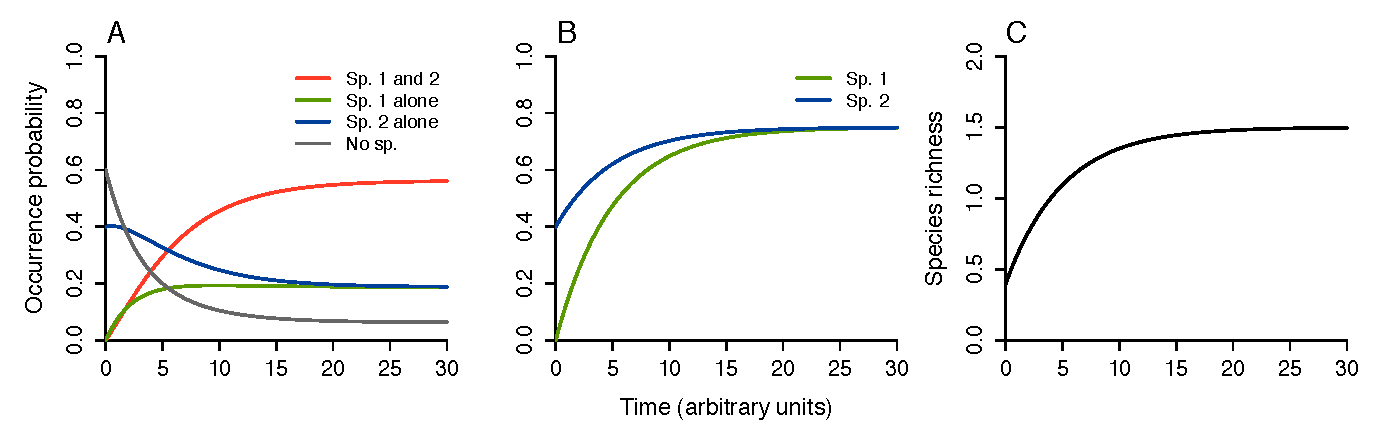
\includegraphics[width=\textwidth]{./annexe3/fig1.eps}
\caption[Simple food webs illustrting the TTTIB]{Simple food webs used to illustrate the TTTIB \cite{Gravel2011}.
 (a) The complete food web (on the mainland) consists in five different species (A,B,C,D,E);
 (b) sub-food webs that species A can colonize; (c) sub-food webs that species A cannot colonize.
}
\label{ann3fig1}
\end{figure}


\begin{table}[]
\centering
\caption[Community states associated to simple networks]{Community states associated to the B-C-D-E network. They are
all the combinations of presence and absence of species. At any time
\(t\), \(C_{t>0}\) represents the species composition of the island and
thus is in one of the sixteen possible \(S_k\) states listed. Here all
communities are considered regardless whether there are TTIB-compatible
as highlighted in the right column.}
\label{tabAnnIII_1}
  \begin{tabular}{|l|l|l|l|l|l|}
    Community states & B & C & D & E & TTIB-compatible \\ \hline
    \(S_{0}\) & 0 & 0 & 0 & 0 & yes \\
    \(S_{1}\) & 0 & 0 & 0 & 1 & no \\
    \(S_{2}\) & 0 & 0 & 1 & 0 & yes \\
    \(S_{3}\) & 0 & 0 & 1 & 1 & yes \\
    \(S_{4}\) & 0 & 1 & 0 & 0 & yes \\
    \(S_{5}\) & 0 & 1 & 0 & 1 & yes \\
    \(S_{6}\) & 0 & 1 & 1 & 0 & yes \\
    \(S_{7}\) & 0 & 1 & 1 & 1 & no \\
    \(S_{8}\) & 1 & 0 & 0 & 0 & no \\
    \(S_{9}\) & 1 & 0 & 0 & 1 & no \\
    \(S_{10}\) & 1 & 0 & 1 & 0 & no \\
    \(S_{11}\) & 1 & 0 & 1 & 1 & yes \\
    \(S_{12}\) & 1 & 1 & 0 & 0 & yes \\
    \(S_{13}\) & 1 & 1 & 0 & 1 & yes \\
    \(S_{14}\) & 1 & 1 & 1 & 0 & yes \\
    \(S_{15}\) & 1 & 1 & 1 & 1 & yes
  \end{tabular}
\end{table}


Deriving the master equation associated to a given community state
\(S_k\) required to study the transition probabilities between community
states between \(t\) and \(t+dt\) (where \(dt\) is assumed to be short enough
to  only one transition). As all the community states are included
in the set \(S_k, k\in\{1,2,...,2^T\}\), following the law of total
probability, for any community states:

\begin{equation}
P_{C_{t+dt}=S_{k}}= \sum_{l=0}^{2^T-1} P_{C_{t+dt}=S_k|C_{t}=S_l}P_{C_{t}=S_l}
\end{equation}

\(P_{C_{t+dt}=S_k|C_{t}=S_l}\) are now assumed to be a linear function
of \(dt\), this assumption is needed valid only for a very small time
step. For \(k \neq l\) :

\begin{equation}
P_{C_{t+dt}=S_k|C_{t}=S_l} = f(S_k,S_l)dt \\
\end{equation}

and, as \(\sum_l P_{C_{t+dt}=S_l|C_{t}=S_k} = 1\) :

\begin{equation}
P_{C_{t+dt}=S_k|C_{t}=S_k} = 1-\sum_{l \neq k}f(S_l,S_k)dt
\end{equation}

\(f(S_k,S_l)\) reflects how easy the transition between \(S_k\) and
\(S_l\) is, it may be greater than one as long as
\(f(S_k,S_l)dt\leqslant1\). The TTIB actually acknowledges the existence
of trophic interactions by assuming :

\begin{enumerate}
\def\labelenumi{\arabic{enumi}.}
\tightlist
\item
  \(f(S_k,S_l)=0\) when the transition from \(S_l\) to \(S_k\) involves
  the colonization of a predator without any prey,
\item
  \(f(S_k,S_l)dt=1\) when \(S_l\) is a community states where a predator
  is present without any prey and \(S_k\) the same community without the
  predator.
\end{enumerate}

Plugging the two latter equations in equation (1) :

\begin{equation}
\frac{P_{C_{t+dt}=S_{k}}-P_{C_{t}=S_{k}}}{dt} = -\left(\sum_{l \neq k}f(S_l,S_k)\right)P_{C_{t}=S_{k}} + \sum_{l \neq k}f(S_k,S_l)P_{C_{t}=S_{l}}
\end{equation}

When \(dt \rightarrow 0\) it provides the master equation than can be
write in in vector format to integrate the dynamic of all community
states \(\mathbf{P}=(P_{S_1}, P_{S_2}, ..., P_{S_{2^T}})\) :

\begin{equation}
\frac{d\mathbf{P}}{dt} = \mathbf{M}\mathbf{P}
\end{equation}

This equation is similar to equation (1.13) but here \(\mathbf{P}\)
includes all the community states and the coefficient of the matrix
\(\mathbf{M}\) depends of the community. Nevertheless the form of the
solution remains equivalent :

\begin{equation}
\mathbf{P}(t) = e^{t\mathbf{M}}\mathbf{P_0}
\end{equation}

This actually describes a continuous-time Markov chain. When all the
community states communicate (\emph{i.e} the Markov chain is
irreducible), their probabilities reached an equilibrium
\(\mathbf{P}^{\*}\) given by the vector in the kernel of \(\mathbf{M}\)
whose elements sum to one.

\section{Reasonable approximations}\label{reasonable-approximations}

The formulation above allows the study of non-independent species
between species but suffers from its generality : for \(T\) species, the
matrix \(\mathbf{M}\) must be filled with \((2^T-1) \times (2^T-1)\)
coefficients (`\(-1\)' acknowledges that for any time \(t\) the elements
of \(\mathbf{P}(t)\) sum to one). Even if the knowledge of a particular
network may help finding these coefficients, reasonable assumptions can
be made to decrease the complexity of \(\mathbf{M}\). First, community
compositions between \(t\) and \(t+dt\) cannot differ in more than one
species, \emph{i.e.} \(f(S_k,S_l)=0\) if \(|S_k-S_l|>1\). This turns
\(\mathbf{M}\) into a sparse matrix : only \(T \times (2^T-1)\) are not
zero. This assumption is not possible in the TTIB as the extinction of a
prey may lead to more than one extinction. However, this issue is easy
to circumvent by allowing the predator to survive a (very) short period
alone one the island. This can be done using large value for
\(f(S_k,S_l)\) that measures the transition of a community with a
predator and the same community without it.

A second hypothesis is that colonization processes may be independent of
interactions. That is, a predator can actually colonize an island
without any prey. This is reasonable if the extinction probability of
this predator on such island is high as recommended to make the first
assumption. Therefore, \(f(S_k,S_l)=c\) when \(sum\{S_k-S_l\}=-1\). The
latter assumption is also useful to integrate variability in dispersal
capacities among species \textbf{{[}Cazelles2015{]}}. Table 4 presents
the matrix \(\mathbf{M}\) for species C, D and E, \emph{i.e.} community
states from \(S_0\) to \(S_8\). Once the colonization probability is
determined, the remaining \(T \times (2^T-2)\) coefficients needed can
be found based on the biological knowledge of species studies,
\emph{e.g.} the nature and the strength of interactions.

\section{Deriving species richness}\label{deriving-species-richness}

The solution \(\mathbf{P}^{\*}\) contains the probabilities of all
community states at equilibrium. This information is actually more than
the knowledge of individual presence and species richness. Indeed these
latter probabilities are particular unions of community states,
therefore \(\mathbf{P}^{\*}\) is sufficient to derive them at
equilibrium. The probability of a species being present at equilibrium
is given by :

\begin{equation}
P_{X_i=1} = \sum_{k \mid S_{k,i}=1} \mathbf{P}_{k}^{\*}
\end{equation}

where \(S_{i,k}\) is the \(i^{th}\) component of \(S_i\) (the one
pertaining to species \(i\)) and \(\mathbf{P}_{i}^{\*}\) the \(k^{th}\)
component of \(\mathbf{P}_{i}\). Similarly, the species richness is
given by the sum of \(\mathbf{P}^{\*}\) weighted by the cardinal of the
community states it refers to:

\begin{equation}
S= \sum_{k=0}^{2^T-1} |S_k|\mathbf{P}_{k}^{\*}
\end{equation}

In a similar fashion, many probabilities can be derived regarding either
a particular set of species either a particular property of the
community. For instance, this framework allows to derive the probability
of finding a given set of predators but also the mean trophic level
expected and even the probability of having a trophic chains of at least
\(p\) levels. In all these situations, the calculus required the
identification of the community states to be summed.

\newpage

\begin{longtable}[]{@{}lllllllll@{}}
\caption{The transition matrix of the Markov chain continuous-time
associated to all combinations of C,D and E species.}\tabularnewline
\toprule
& \(S_{0}\) & \(S_{1}\) & \(S_{2}\) & \(S_{3}\) & \(S_{4}\) & \(S_{5}\)
& \(S_{6}\) & \(S_{7}\)\tabularnewline
\midrule
\endfirsthead
\toprule
& \(S_{0}\) & \(S_{1}\) & \(S_{2}\) & \(S_{3}\) & \(S_{4}\) & \(S_{5}\)
& \(S_{6}\) & \(S_{7}\)\tabularnewline
\midrule
\endhead
\(S_{0}\) & \(1-c-c-c\) & \(f(S_{1},S_{,0})\) & \(f(S_{2},S_{,0})\) & &
\(f(S_{4},S_{,0})\) & & &\tabularnewline
\(S_{1}\) & \(c\) & \(1-f(S_{1},S_{,0})-c-c\) & & \(f(S_{3},S_{,1})\) &
& \(f(S_{5},S_{,1})\) & &\tabularnewline
\(S_{2}\) & \(c\) & & \(1-f(S_{2},S_{,0})-c-c\) & \(f(S_{3},S_{,2})\) &
& & \(f(S_{6},S_{,2})\) &\tabularnewline
\(S_{3}\) & & \(c\) & \(c\) & \(1-f(S_{3},S_{,1})-f(S_{3},S_{,2})-c\) &
& & & \(f(S_{7},S_{,3})\)\tabularnewline
\(S_{4}\) & \(c\) & & & & \(1-f(S_{4},S_{,0})-c-c\) &
\(f(S_{5},S_{,4})\) & \(f(S_{6},S_{,4})\) &\tabularnewline
\(S_{5}\) & & \(c\) & & & \(c\) &
\(1-f(S_{5},S_{,1})-f(S_{5},S_{,4})-c\) & &
\(f(S_{7},S_{,5})\)\tabularnewline
\(S_{6}\) & & & \(c\) & & \(c\) & &
\(1-f(S_{6},S_{,2})-f(S_{6},S_{,4})-c\) &
\(f(S_{7},S_{,6})\)\tabularnewline
\(S_{7}\) & & & & \(c\) & & \(c\) & \(c\) &
\(1-f(S_{7},S_{,3})-f(S_{7},S_{,5})-f(S_{7},S_{,6})\)\tabularnewline
\bottomrule
\end{longtable}
